\subsection{Double Exponent Model}

Let us look at the input:

\begin{equation}
    I(t) = I_0 \cdot e^{-t/\tau_s}
\end{equation}

For our old familiar differential:

\begin{equation}
    v(t) + \tau_m \cdot \dot{v}(t) = I(t)
\end{equation}

The solution will look like:

\begin{equation}
    v(t) = A \cdot e^{-t/\tau_m} + B \cdot e^{-t/\tau_s}
\end{equation}

We can normalize it into:

\begin{equation}
    v(t) = v_0 \cdot (e^{-t/\tau_m} - e^{-t/\tau_s})
\end{equation}

\begin{figure}[H]
    \centering
    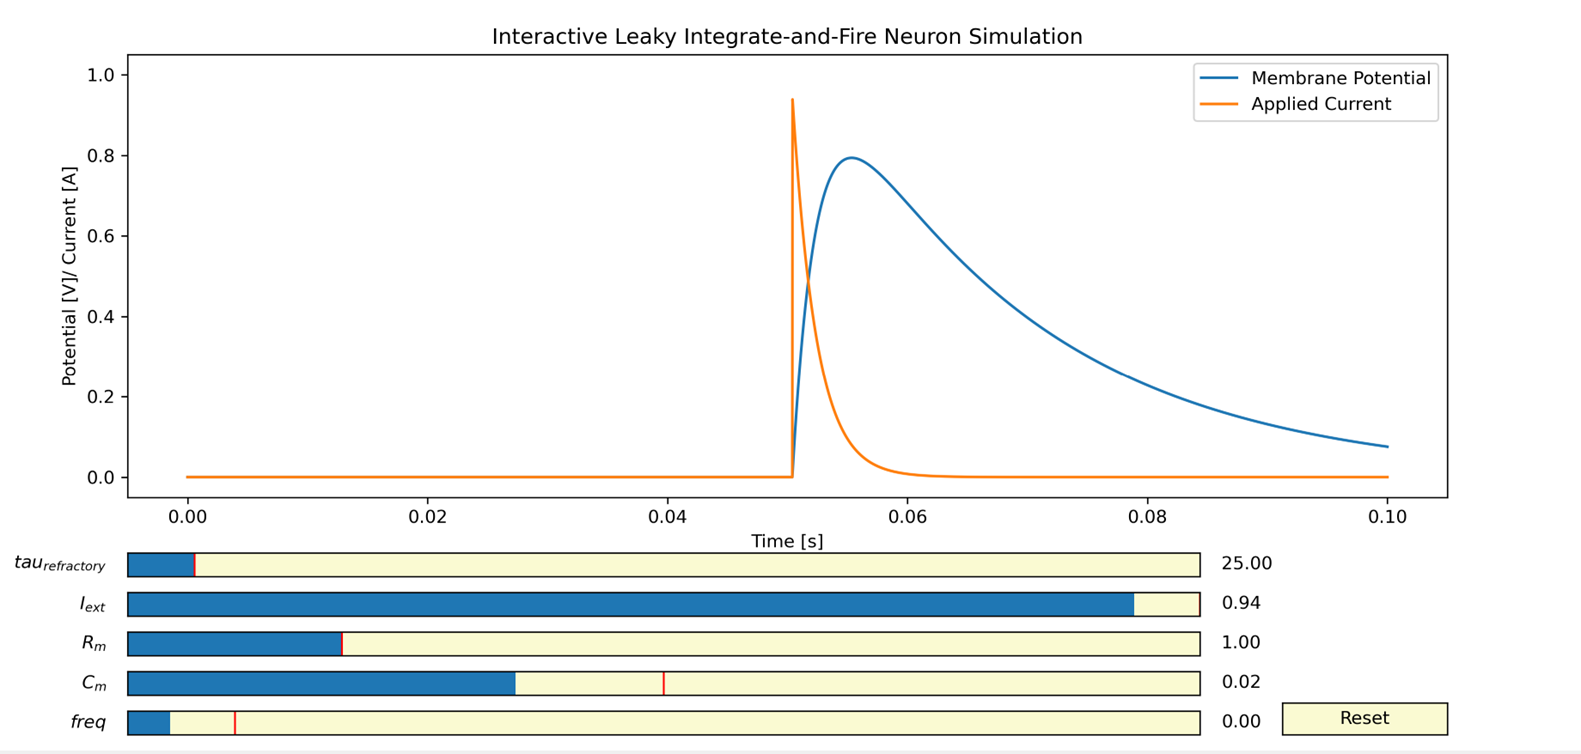
\includegraphics[width=0.8\textwidth]{methods/computational-models/graphs/LIF-second-order.png}
    \caption{LIF 2-order membrane voltage response to spike}
    \label{fig:LIF-second-order}
\end{figure}

A useful definition will be:

\begin{equation}
    k(t) = v_0 \cdot (e^{-t/\tau_m} - e^{-t/\tau_s})
\end{equation}

So, the solution for:

\begin{equation}
    v(t) = \sum_{t^l} k(t - t^l)
\end{equation}

\begin{figure}[H]
    \centering
    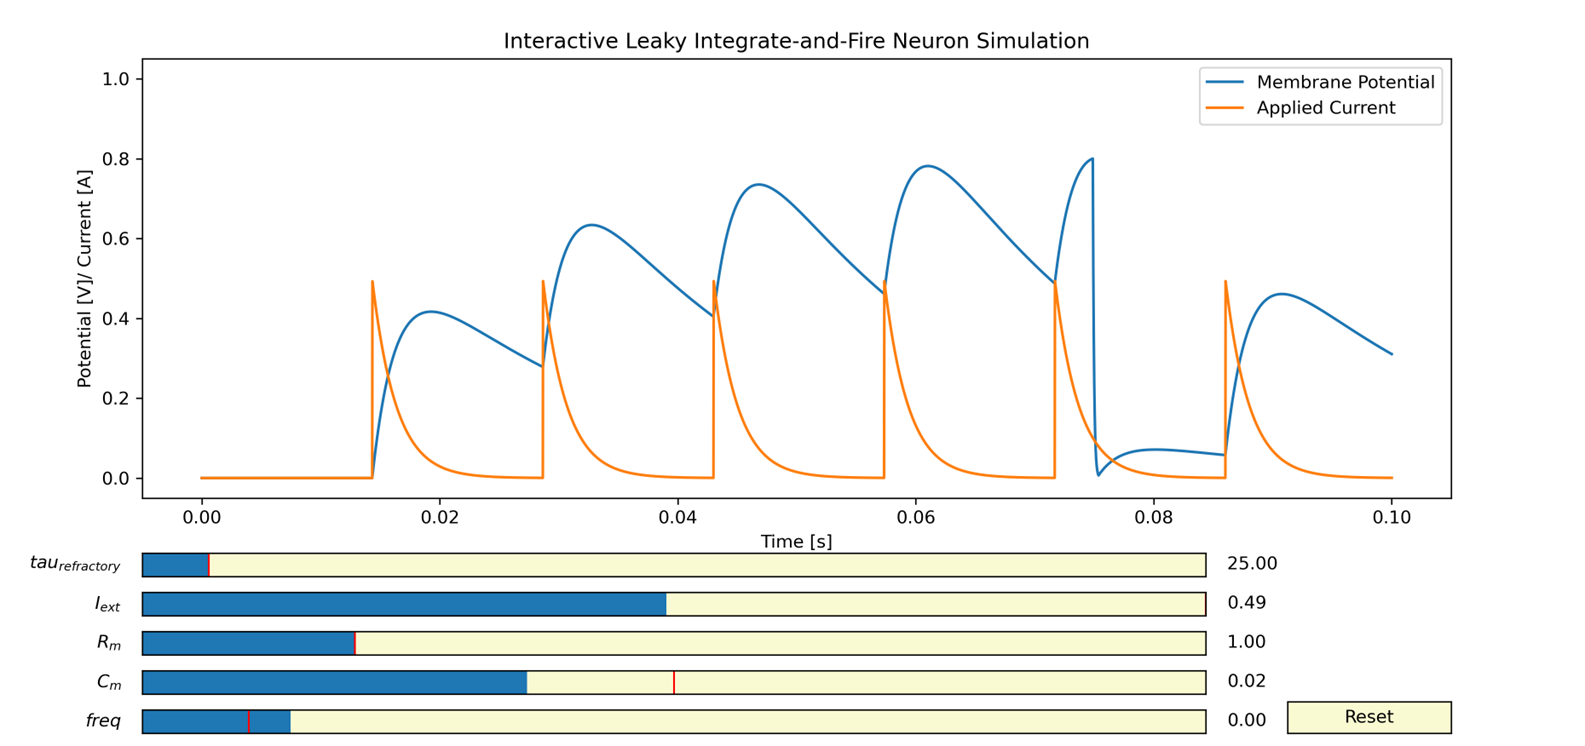
\includegraphics[width=0.8\textwidth]{methods/computational-models/graphs/LIF-spike-response-second-order.png}
    \caption{LIF 2-order membrane voltage response to multiple spikes}
    \label{fig:LIF-second-order-spike-response}
\end{figure}
